\documentclass[11pt,twoside,titlepage]{article}
\usepackage[tc]{titlepic}
\usepackage{times}
\usepackage{float}
\usepackage{amssymb}
\usepackage{amsmath}
\usepackage{amsthm}
\usepackage{needspace}
\usepackage{url}
\usepackage{hyperref}
%\usepackage{mathptm}
\usepackage{fancyhdr}
\usepackage{wrapfig}
\ifx\pdfoutput\undefined
% we are running LaTeX, not pdflatex
\usepackage{epsfig,color}
\else
% we are running pdflatex, so convert .eps files to .pdf
\usepackage[pdftex]{epsfig,color}
\usepackage{epstopdf}
\usepackage{pdfsync}
\fi
\usepackage{ifthen,version}
\usepackage{listings}
%\usepackage{temporal}
%\usepackage{algorithmic}
\newboolean{print-solutions}

% Start of configuration section
% Comment out the following line to exclude the printing of solutions.
%\setboolean{print-solutions}{true}
\newcommand{\labnumber}{1}
\newcommand{\labname}{Digital Logic Gates}
\newcommand{\coursenumber}{Vivado 2018.3 Installation How-To Document}
\newcommand{\coursename}{Introduction to Digital Design}
% End of configuration section

% Conditional definitions
\newcommand{\dateorsol}{\LARGE \ifthenelse{\boolean{print-solutions}}%
  {Solutions}{Due \duedate}}
\newcommand{\headertxt}{\sl \ifthenelse{\boolean{print-solutions}}%
  {Solutions to}{} Laboratory Exercise \#\labnumber}
\newcommand{\points}[1]{\ifthenelse{\boolean{print-solutions}}%
  {}{[#1 points.]}}
\ifthenelse{\boolean{print-solutions}}{\includeversion{prnt-solns}}%
{\excludeversion{prnt-solns}}

\textwidth=7.25in
\evensidemargin=-0.35in
\oddsidemargin=-0.35in

\newcommand{\ite}{\operatorname{ite}}
\newcommand{\itec}{\operatorname{ite\_constant}}

{\theoremstyle{definition} \newtheorem{definition}{Definition}}
\newtheorem{theorem}{Theorem}
\newtheorem{lemma}{Lemma}
\newtheorem{corollary}{Corollary}
\newtheorem{proposition}{Proposition}
{\theoremstyle{remark}
  \newtheorem{example}{Example}
  \newtheorem{problem}{Problem}
  \newtheorem{note}{Note}}
% Fortunately, proofs can be nested.
\newenvironment{solution}{\begin{proof}[Solution]}{\end{proof}}


\newcommand{\ta}{Created By: Kyler Scott and Prof. Sunil P. Khatri\\July 2020}
\title{ \huge Department of Electrical and Computer Engineering\\ \huge Texas A\&M University \\}
\author{ \huge Vivado 2018.3 Installation:\\ \\ \huge How-To Document \\ \\ \\ \ta}

\titlepic{
\includegraphics[width=0.5\textwidth]{logo}}

\date{}
\pagestyle{fancy}
\lhead[\rm\thepage]{}
\rhead[]{\rm\thepage}
\lfoot[]{\coursenumber}
%\cfoot{\instructor}
\rfoot[\coursenumber]{}

\begin{document}
\bibliographystyle{alpha}
\maketitle

\noindent
\textbf{Note:} This guide is intended for students running the Windows OS. If you are a Mac user, you must first set up an instance of the Windows OS on your Mac. For this, refer to the "Bootcamp How-To Document" for instructions on how to use Bootcamp to run Windows OS on your Mac machine. After you are running the Windows OS, you can follow the steps described in this document to install Vivado 2018.3.\\

\noindent
\textbf{Note:} Before you begin the Vivado 2018.3 installation, be sure that you have enough free disk space. The installation alone will require 33GB, and you will need space left over for the files generated while completing the labs. It is therefore recommended that you have at least 40GB of free disk space before starting this installation.\\

\section{Introduction}
Students completing the ECEN 248 or ECEN 449/749 labs will be required to download Vivado 2018.3 onto their local computer. This guide will provide installation instructions for Vivado 2018.3 that are specific to the ECEN 248 and ECEN 449/749 labs.

\section{Installation}

Open a web browser and go to the \href{https://www.xilinx.com/support/download/index.html/content/xilinx/en/downloadNav/vivado-design-tools/2018-3.html}{Vivado downloads page}. Make sure version 2018.3 is selected on the left panel. Scroll down to "Vivado Design Suite -  HLx Editions - 2018.3" and click the link that says "Vivado HLx 2018.3: WebPACK and Editions - Windows Self Extracting Web Installer" as shown in Figure~\ref{install}.\\

\begin{figure}[!h]
	\centering 
	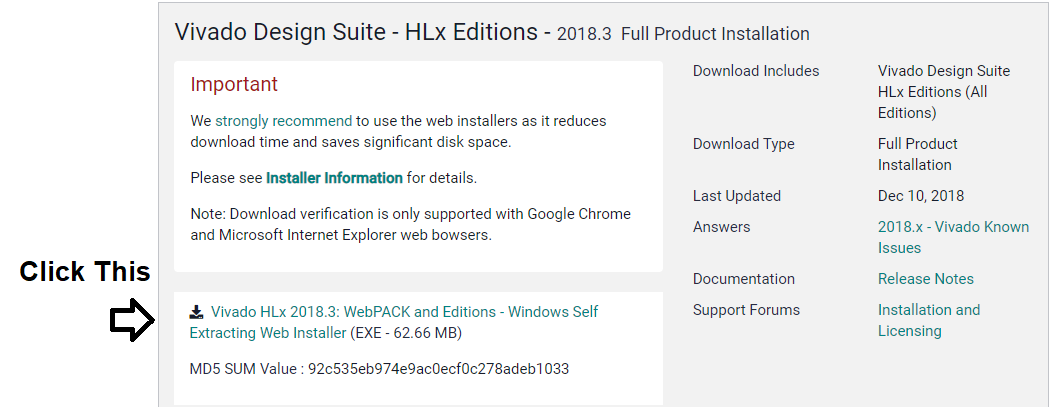
\includegraphics[ width=.8\textwidth]{install}
	\caption{Click to Download the Windows Self Extracting Web Installer}
	\label{install}
\end{figure}

\noindent
In order to download the installer, you will need a Xilinx account. When you try to download the installer it will prompt you to log in or create an account. If you do not have an account, create one at this step or log in if you already have one. You will need to log in again later when you run the installer. After signing in it will prompt you to enter some personal information before downloading the installer. Enter the information and click "Download" to begin the download. \\

\noindent
This will download a .exe file. Once the download is complete, navigate to the file and run it. This will open a window that looks like Figure~\ref{installer}. Click "Next", and enter your Xilinx account login info. Be sure the "Download and Install Now" button is selected and click "Next". Agree to the license agreements and click "Next". Select "Vivado HL Design Edition" and click "Next".\\

\begin{figure}[!h]
	\centering 
	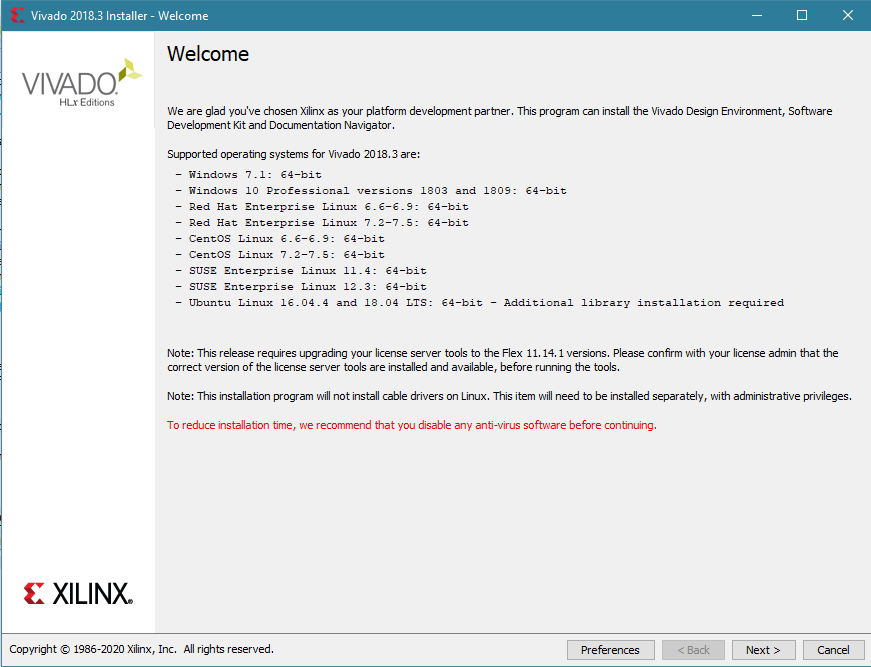
\includegraphics[ width=.8\textwidth]{installer}
	\caption{Windows Self Extracting Web Installer}
	\label{installer}
\end{figure}

\noindent
On the next page, under Devices $\rightarrow$ Production Devices, deselect "7 Series", "UltraScale" and "UltraScale+". These are all devices that we will not be using in ECEN 248 or ECEN 449/749 labs, and so we can deselect them to decrease the amount of disk space this installation uses. Your screen should look like Figure~\ref{boards}. \\

\begin{figure}[!h]
	\centering 
	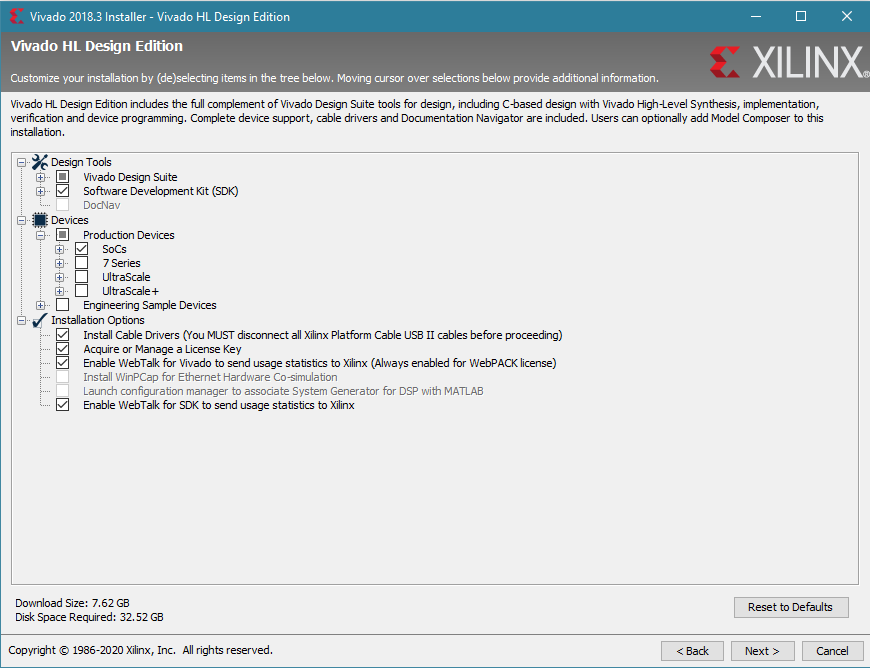
\includegraphics[ width=.8\textwidth]{boards}
	\caption{Vivado HL Design Edition: Custom Installation}
	\label{boards}
\end{figure}

\noindent
On the next page, select a location for the installation and click "Next". Then click "Install" to begin the installation. This may take more than an hour to complete.\\

\end{document}

